Before moving on to the Modeling section, we first define the tire parameters. We assume both tires have an equal weight of 9 kg. The radius of the rear tire, denoted as $a$, is 0.33 m, and the radius of the front tire, denoted as $c$, is also 0.33 m. Using these values, we can calculate the height $h$. As previously mentioned, the values of $H$ and $h$ can be considered equal.
\begin{equation*}
	h = CoG - r_a \approx CoG - r_c = H
\end{equation*} 
Since all of the variables are known, we can proceed to calculate the values of $A$, $B$, $C$ and $D$ (s. \ref{sec: The_mod} Theoretical Model) for each drive type. In our model value $B$ is negligible, as there's no corresponding values. This steams from the simplicity of the model.
\subsubsection*{Tractive Power \& Power}
	The tractive force is the force produced by the vehicle's propulsion system to initiate and sustain its motion. Force, on its own, does not provide any meaningful information about the energy or work performed by the system. Hence, we need to introduce Tractive Power:
	\begin{equation*}
		P_T(t) = F_T(t)\cdot\dot x = \left( A + B\dot x + C\dot x^2 + D\ddot x \right)\cdot\dot x.
	\end{equation*}
	The tractive power, just like the tractive force, only considers the power required to propel the vehicle forward, while other components need to be accounted for as well.
	$P_{\text{HVAC}}$ represents the power consumed by the heating, ventilation, and air conditioning system, which we estimate to be around 1.5 kW. We assume 
	\begin{equation*}
		P(t) = \left( A + B\dot x + C\dot x^2 + D\ddot x\right)\cdot\dot x + P_{\text{HVAC}}
	\end{equation*}
	We assume the engine remains active during standby, so $P_{\text{HVAC}}$ is included. The zero-velocity periods are too brief to suggest the vehicle is off.
	The figures below show the Tractive Force and Power profiles for each drive cycle.
	\begin{figure}[H]
		\begin{center}
			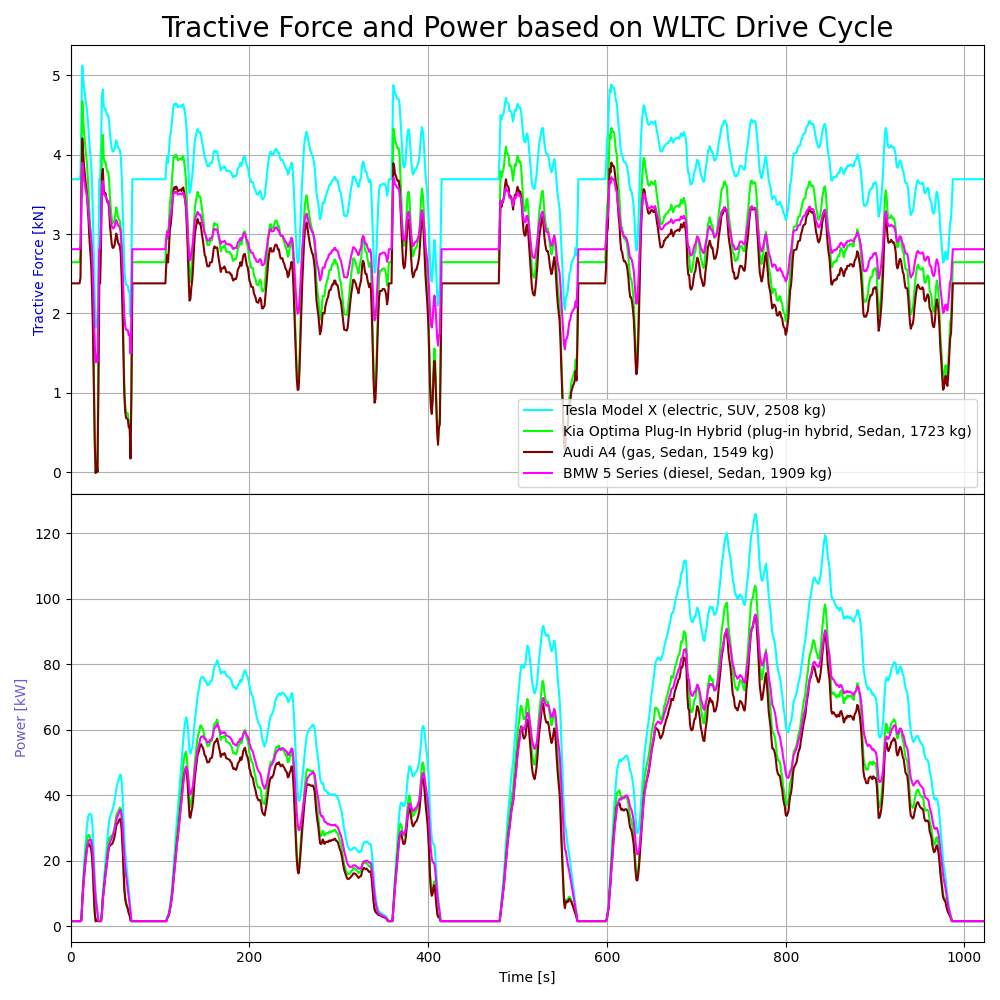
\includegraphics[width=\linewidth]{images/Tractives_WLTC.png}
			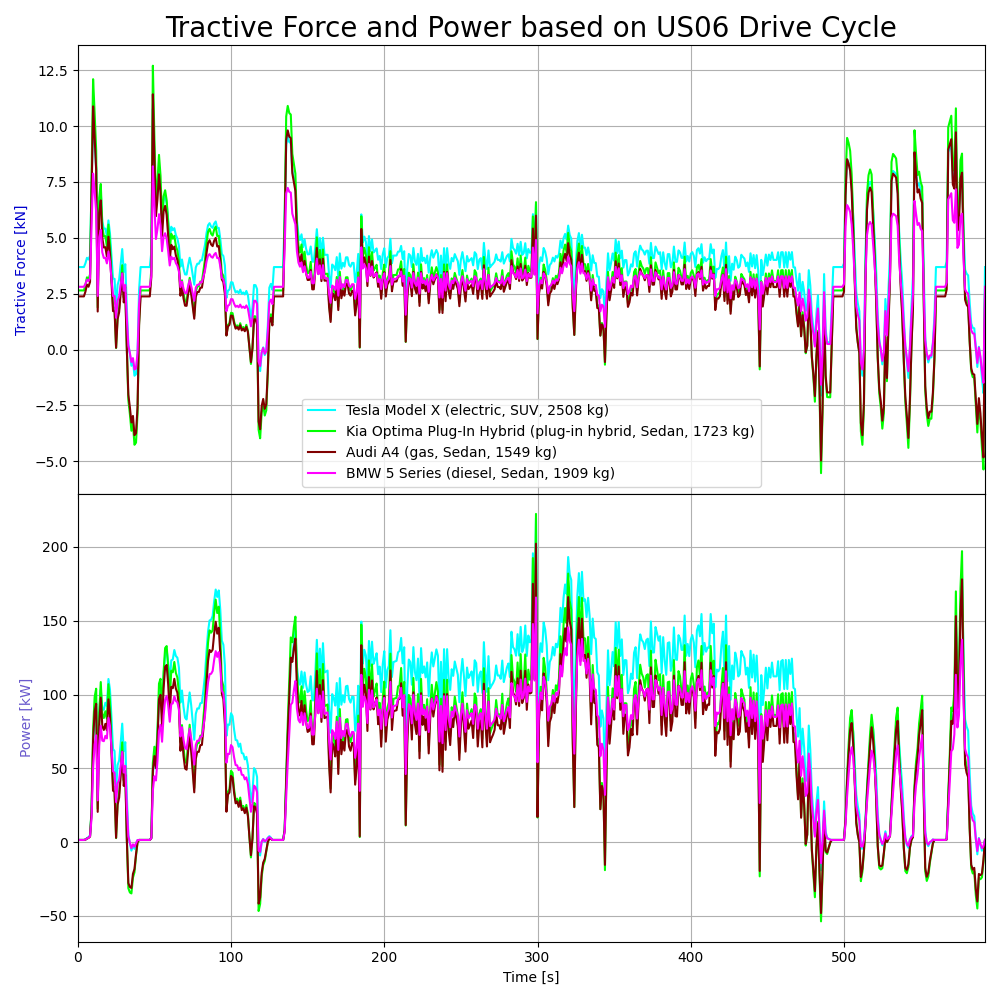
\includegraphics[width=\linewidth]{images/Tractives_US06.png}
			\caption{Tractive Force and Power Profiles}
		\end{center}
	\end{figure}
\subsubsection*{Efficiency \& Energy}
	Energy losses due to friction and electrical components are inevitable, so we use efficiency ratios to quantify these losses. These ratios compare the actual state with the ideal state. Key efficiencies are:
	\begin{align*}
		\text{Regenerative Braking:} && \eta_{\text{reg}} = \frac{P_{\text{reg}}}{P_{\text{brake}}} & = \frac{P_{\text{reg}}}{P_T}, \\
		\text{Powertrain:} && \eta_{\text{pt}} = \frac{P}{P_{\text{motor}}} & = \frac{P}{P_{b}}, \\
		\text{Fuel-to-Wheel:} && \eta_{\text{F-W}} & = \frac{P_T}{P_{\text{F-W}}}.
	\end{align*}
	The Regenerative Braking Efficiency $\eta_{\text{reg}}$ compares the power recovered during braking $P_{\text{reg}}$ to the tractive power $P_T$, as the energy recovery occurs through the same propulsion system.
			
	Powertrain efficiency $\eta_{\text{pt}}$ compares the Total Power $P$ to the power drawn from the battery $P_b$. It reflects the efficiency of components transmitting energy from the battery to the wheels, considering both propulsion and auxiliary systems. Hence, the total power $P$ is used. Since $P_{\text{motor}}$ equals $P_b$, both terms are interchangeable.
	
	For many modeling purposes, tank-to-wheel efficiency is commonly approximated as a constant. However, this efficiency depends on a range of operational characteristics and is not inherently fixed. In this study, we adopt the value utility parameter $p=0.2$, which represents the average proportion of the engine’s maximum work capacity utilized throughout the drive cycle. This value is derived from simulated data and taken from Figure 4 of the cited paper. Based on this, we assume fuel-to-wheel efficiencies of 27\% for gasoline and 30\% for diesel vehicles, and a powertrain efficiency of 75\%. \cite{HJELKREM2020115463}
	
	For the Mitsubishi i-MiEV, data has shown that the regenerative braking system (RBS) can recover up to 62\% of the available kinetic energy under ideal conditions, such as at a speed of 120 km/h over a short interval. However, regenerative performance varies significantly depending on the drive cycle and vehicle settings. Based on typical cycle characteristics and findings from comparable studies, we assume a regenerative braking efficiency of 45\% for the WLTC drive cycle, which includes a balanced mix of urban and highway segments, and 35\% for the US06 drive cycle, which features more aggressive acceleration and braking. These values reflect realistic average efficiencies for electric vehicles operating under these respective conditions. \parencite[p. 1423]{doi:10.1177/0954407017728651}
	
	The total power $P$ can be divided into Motoring Power $P_{\text{motor}}$, which draws energy from the battery ($P_b$), and Braking Power $P_{\text{brake}}$. Braking occurs when acceleration and velocity are in opposite directions, while motoring occurs when they are in the same direction.
	\begin{equation*}
		P(t) = \left\{  
			\begin{array}{cc} 
				P_{motor},  & \dot x \cdot \ddot x \geq 0 \\
				P_{brake},  & \dot x \cdot \ddot x < 0  
			\end{array} \right.
	\end{equation*}
	To propel the vehicle, motoring energy $W_{\text{motor}}$ must be supplied. During braking, electric and hybrid vehicles recover energy $W_{\text{brake}}$, while conventional vehicles do not.
	\begin{align*}
		W_b & = \int P_{b} dt = \int \frac{P}{\eta_{\text{pt}}}dt = \int P_{\text{motor}} dt = W_{\text{motor}}\\
		W_{\text{reg}} & = \int P_{\text{reg}} dt =\eta_{\text{reg}}\int P_{T} dt = \eta_{\text{reg}} W_{\text{brake}} 
	\end{align*}
\subsubsection*{Hybrid Vehicles}
	Electric and conventional vehicles rely solely on electric motors and internal combustion engines, respectively. Hybrid vehiclesq, on the other hand, alternate between both power sources.
	
	Hybrid vehicles typically use their electric motor during vehicle launch (below 16 km/h), light acceleration (assumed less than 2 m/s$^2$), and regenerative braking (mild deceleration). The combustion engine engages at cruising speeds above 50 km/h, under strong acceleration, or when the battery’s state of charge is low (below 20\%). \cite{burke2000lesson}

	The algorithms developed to determine the engine mode condition and compute the energy consumption for hybrid vehicles are provided in \ref{sec: apx} Appendix as Algorithm \ref{alg: hyb_cond} and Algorithm \ref{alg: hyb_energy}, respectively.

	\begin{figure}[H]
		\begin{center}
			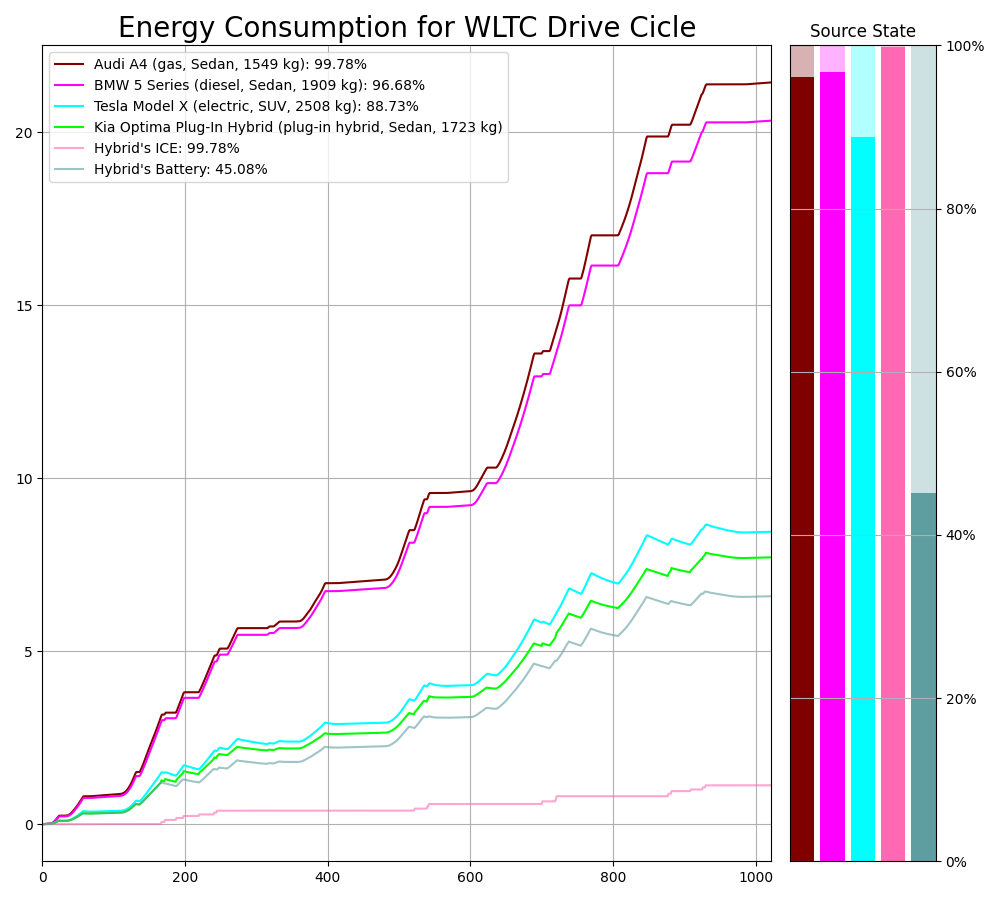
\includegraphics[scale=.33]{W_WLTC.png}
			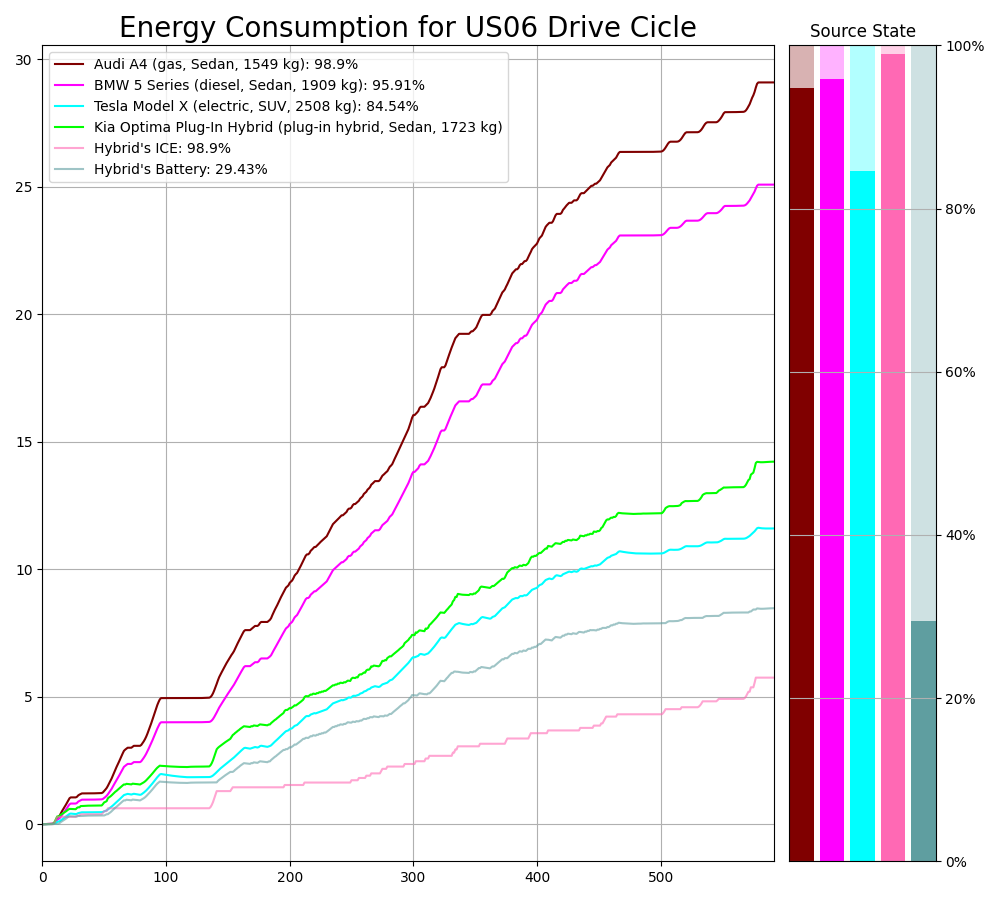
\includegraphics[scale=.33]{W_US06.png}
		\end{center}
		\caption{Energy Consumption Across Drive Cycles for Different Powertrains}
	\end{figure}
		
\subsection*{Fuel Consumption}
	Fuel consumption refers to the amount of fuel a vehicle uses to travel a specific distance, commonly expressed in liters per 100 kilometers or miles per gallon. It reflects the vehicle’s energy efficiency and is influenced by factors such as driving behavior, engine type, vehicle load, and environmental conditions. To allow for consistent comparison across internal combustion engine vehicles, hybrids, and electric vehicles, all fuel consumption values in this study are converted and expressed in kilowatt-hours per kilometer (kWh/km).
	\begin{equation*}
		FC = \frac{W_{\text{drive}}}{S} = \frac{P_{\text{drive}}}{\dot x}
	\end{equation*}
	\begin{figure}[H]
		\begin{center}
			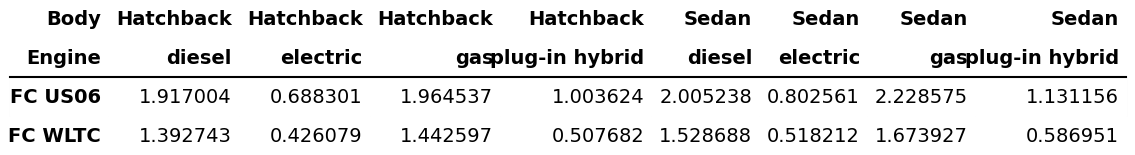
\includegraphics[width=\linewidth]{FC1.png}
			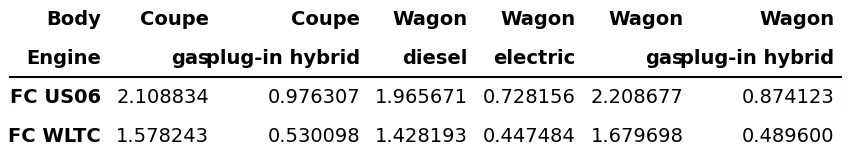
\includegraphics[width=.75\linewidth]{FC2.png}
			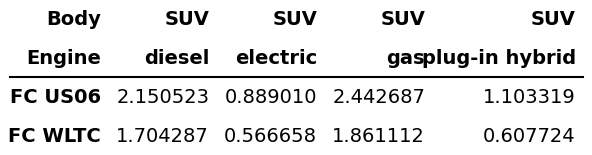
\includegraphics[width=.6\linewidth]{FC3.png}
		\end{center}
		\caption{Fuel Consumption's Mean by Body and Engine Type}
		\label{fig: FC}
	\end{figure}
		Figure \ref{fig: FC} shows the average fuel consumption, categorized by body and engine type. For each entry, the fuel consumption is higher for the US06 drive cycle, which is consistent with its characteristic: higher average speeds result in greater fuel consumption, as visible in Table \ref{tab: drive_cycle}. What about overall representation?
		
		Figure \ref{fig: final} presents the distribution of fuel consumption across all engine types, grouped by vehicle body type. This classification enables a more balanced comparison between vehicles with similar mass distribution and dynamic characteristics. It’s worth noting that data is limited for certain body types, particularly Wagons and Coupes, which are represented by only a few samples or even just two vehicles.
		
		Despite this, clear clustering patterns emerge within each body type based on engine type. Both drive cycles reveal consistently lower fuel consumption for hybrid and electric vehicles across all categories. Notably, none of the electric or hybrid vehicles exceed 1 kWh/km in the WLTC cycle. In contrast, conventional vehicles tend to cluster just below 2 kWh/km.
		
		Under the demanding US06 drive cycle, the differences become even more pronounced. Fuel consumption for conventional SUVs and sedans peaks slightly above 3.5 kWh/km. In comparison, the highest-consuming hybrid remains below 1.5 kWh/km, while electric vehicles top out at just 1 kWh/km.		
	\begin{figure}[H]
		\begin{center}
			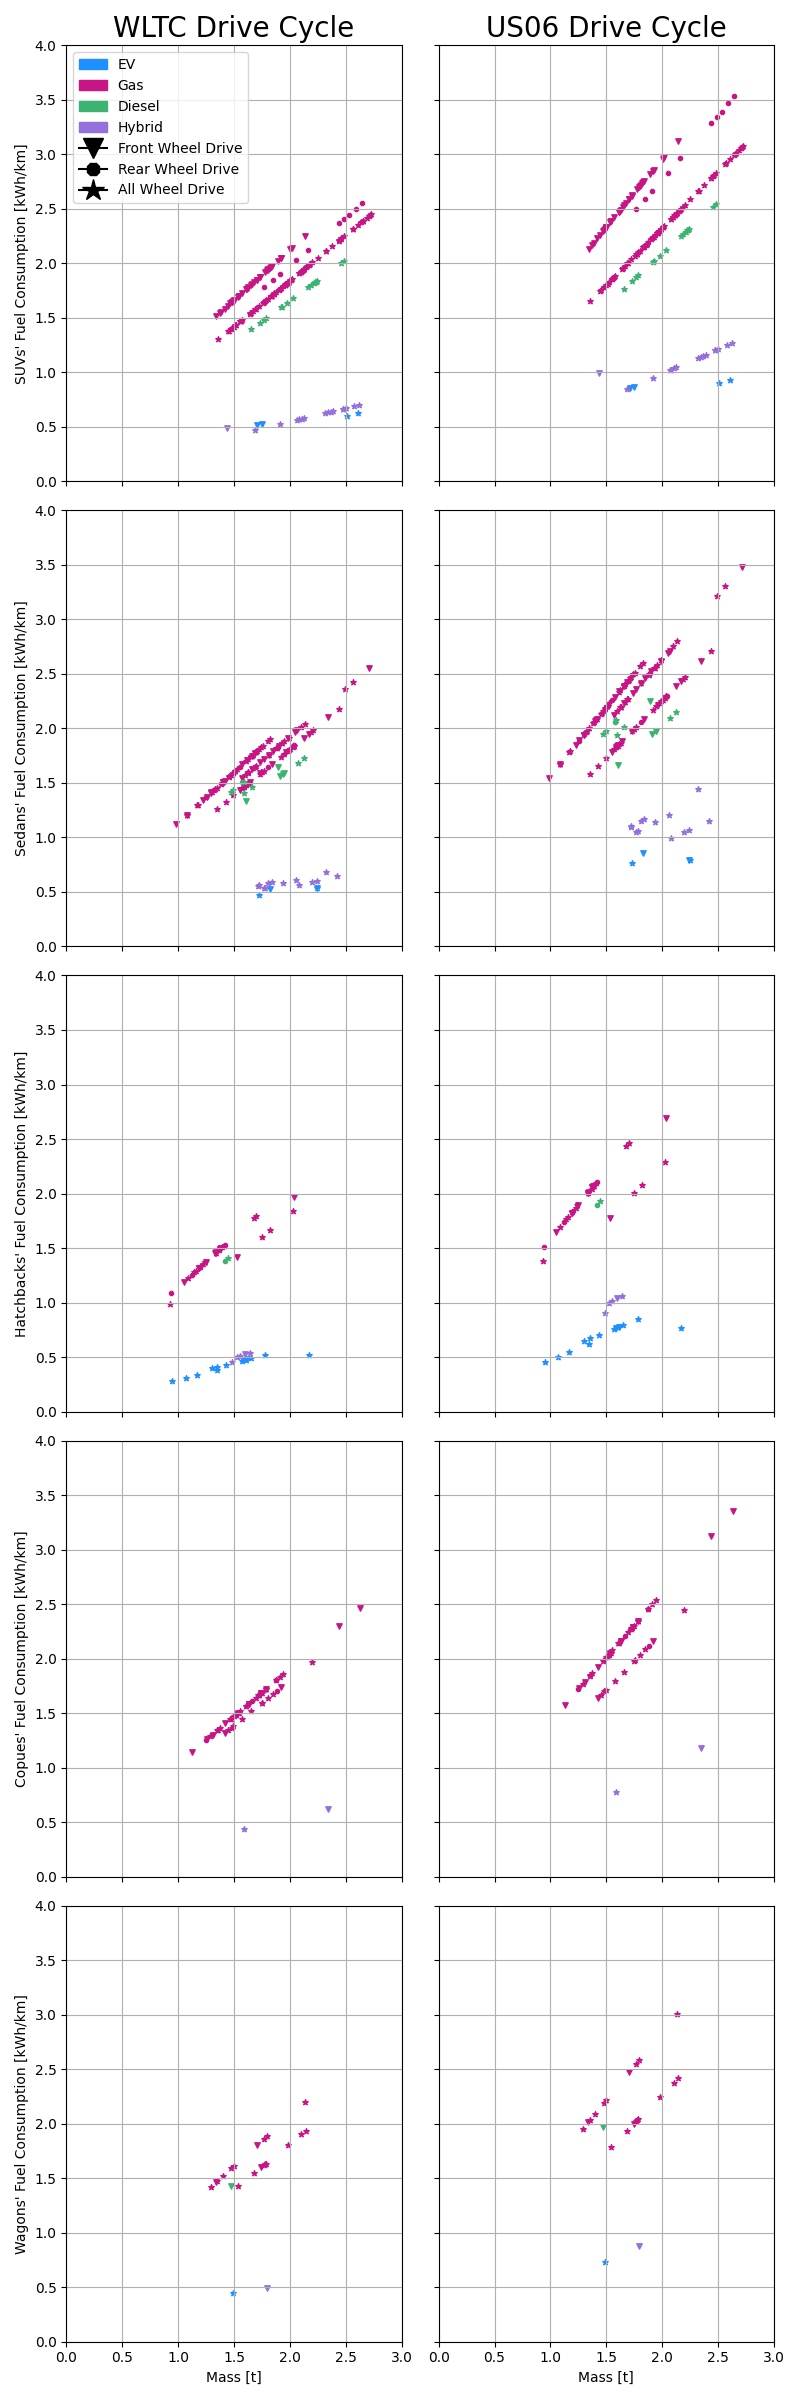
\includegraphics[width=.9\linewidth]{Final.png}
		\end{center}
		\caption{Fuel Consumption by vehicles}
		\label{fig: final}
	\end{figure}
	Let's compute the percentage difference between electric vehicles and the other engine types. We start by sorting the grouped values to identify the maximum and minimum fuel consumption within each category. Then, we calculate the relative efficiency gain of electric vehicles compared to the others. Figure \ref{fig: FC_min_max} highlights the minimum and maximum fuel consumption values across all configurations, while Figure \ref{fig: percent} illustrates how much lower the consumption of electric vehicles is compared to other engine types.
	\begin{figure}[H]
		\begin{multicols}{2}
			\begin{center}
				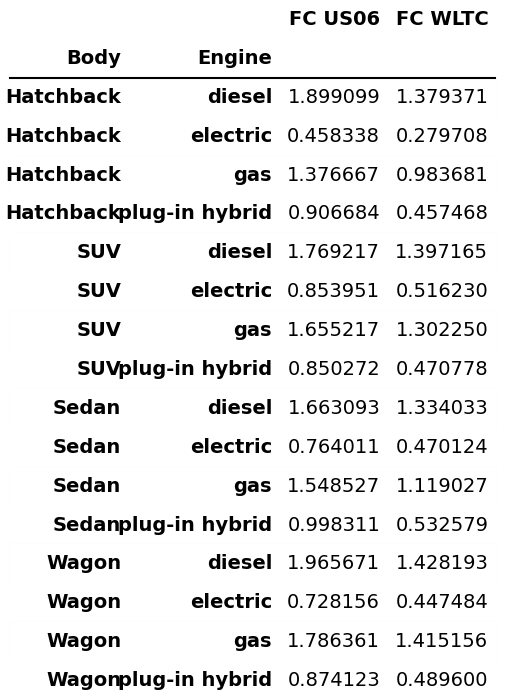
\includegraphics[width=\linewidth]{FCmin.png}
				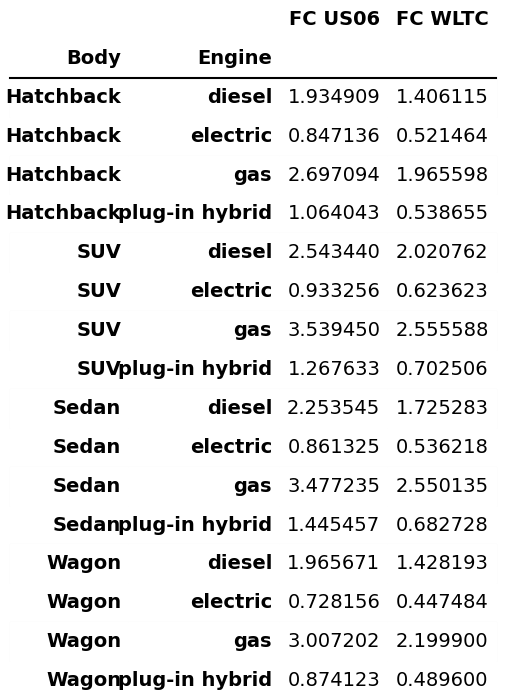
\includegraphics[width=\linewidth]{FCmax.png}
			\end{center}
		\end{multicols}
		\caption{Minimum (left) and Maximum (right) Values of Fuel Consumption grouped by Body and Engine Type}
		\label{fig: FC_min_max}
	\end{figure}
	The percentage gain has been calculated by using the following formula:
	\begin{equation*}
		\text{Gain} = \frac{\text{FC}_{\text{other}} - \text{FC}_{\text{EV}}}{\text{FC}_{\text{other}}} \cdot 100\%
	\end{equation*}
	\begin{figure}[H]
		\begin{multicols}{2}
			\begin{center}
				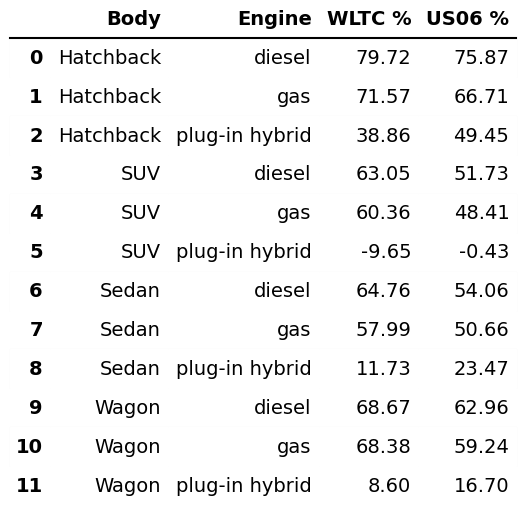
\includegraphics[width=\linewidth]{FCminpercent.png}
				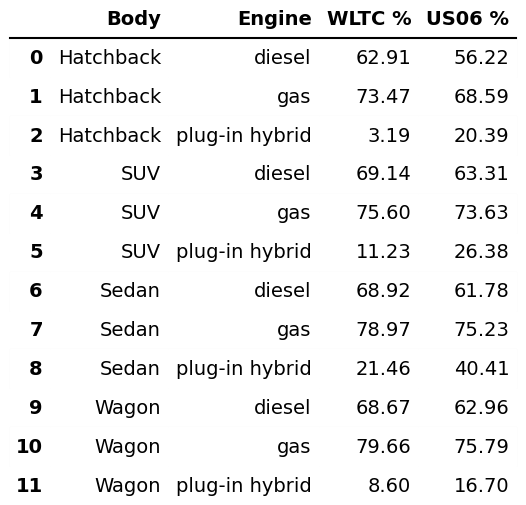
\includegraphics[width=\linewidth]{FCmaxpercent.png}
			\end{center}
		\end{multicols}
		\caption{Minimum (left) and Maximum (right) Percentage Gain of Fuel Consumption grouped by Body and Engine Type}
		\label{fig: percent}
	\end{figure}
	As shown in Figure \ref{fig: percent}, electric vehicles are approximately 63.01\% to 77.63\% more efficient than diesel-powered vehicles, and 57.99\% to 79.66\% more efficient than gasoline-powered vehicles in the WLTC cycle. For hybrid vehicles, the maximum efficiency gain compared to EVs reaches 32.54\%, while the lowest value is -9.65\%—indicating that one hybrid vehicle is actually 9.65\% more efficient than its electric counterpart under the WLTC cycle.
	
	Electric vehicles are approximately 51.73\% to 73.40\% more efficient than diesel-powered vehicles, and 48.41\% to 75.79\% more efficient than gasoline-powered vehicles under the US06 drive cycle. In comparison, hybrid vehicles show a maximum efficiency gain of 44.29\% relative to EVs, while the minimum value is -0.43\% - indicating that one hybrid vehicle is slightly more efficient than an electric vehicle in this particular cycle.
